\documentclass{homework}

\title{Final Exam}
\author{Kevin Evans}
\studentid{11571810}
\date{April 29, 2022}
\setclass{Physics}{465}
\usepackage{amssymb}
\usepackage{mathtools}
\usepackage{amsthm}
\usepackage{amsmath}
\usepackage{physics}
\usepackage{booktabs}
\usepackage{multirow}
\usepackage[inter-unit-product =\cdot]{siunitx}

\usepackage{times}
\usepackage{mhchem}
\usepackage{tikz}

\usepackage[compat=1.1.0]{tikz-feynman}
%\usepackage{calligra}
%\DeclareMathAlphabet{\mathcalligra}{T1}{calligra}{m}{n}
%\DeclareFontShape{T1}{calligra}{m}{n}{<->s*[2.2]callig15}{}
%\newcommand{\scriptr}{\mathcalligra{r}\,}
%\newcommand{\boldscriptr}{\pmb{\mathcalligra{r}}\,}
%\newcommand{\emf}{\mathcal{E}}

\DeclareSIUnit\eVperc{\eV\per\clight}
\DeclareSIUnit\clight{\text{\ensuremath{c}}}
\DeclareSIUnit\year{yr}
\newcommand{\M}{\ensuremath{\mathcal{M}}}
\newcommand{\fm}{\femto\meter}

\renewcommand{\P}{\ensuremath{\mathbb{P}}}

\newcommand{\solution}{	\vspace{1em} \textit{Solution.} \quad }

\begin{document}
	\maketitle
	\begin{enumerate}
		\item Given the charge distribution $$\rho(r) = \rho_0 e^{-r/a} / r,$$
		and using Table 3.1 (since it's spherically symmetric), the form factor is \begin{align*}
			F(q^2) & = \frac{4 \pi \hbar}{Zeq} \int \rho(r) r \sin(qr/\hbar) \dd{r} \\
				& =  \frac{4 \pi \hbar \rho_0}{Zeq} \int_0^\infty e^{-r/a} \sin(q r / \hbar) \dd{r}
			\intertext{Using a definite integration table,}
			F(q^2) & = \frac{4 \pi \hbar \rho_0}{Zeq} \left[
				\frac{q/\hbar}{1/a^2 + (q/\hbar)^2}
			\right] \\
				& =  \frac{4 \pi \rho_0}{Ze}  \frac{1}{1/a^2 + (q/\hbar)^2}.
				%%%%% TODO: check this, since wolfram gives a different FT?
		\end{align*}
	
		\item \begin{enumerate}
			\item In this problem, we've got: \begin{align*}
				\pi & \to \nu + \mu.
				\intertext{In terms of the 4-momenta,}
				\P_\pi & = \P_\nu + \P_\mu \\
%				(m_\pi, 0) & = \P_\nu + (E_\mu, p_\mu) \\
				\implies {\P_\nu}^2 & = \P_\pi^2 - \P_\mu^2 - 2 \P_\pi \cdot \P_\mu \\
					0 & = m_\pi^2 + m_\mu^2 - 2 (m_\pi, 0) \cdot (E_\mu, \bvec{p}_\mu) = m_\pi^2 - m_\mu^2 - 2 E_\mu m_\pi\\
				\implies E_\mu & = \frac{m_\pi^2 + m_\mu^2}{2 m_\pi}.
			\end{align*}
		
			\item From the energy-momentum relation, \begin{align*}
				E_\mu^2 & = p_\mu^2 + m_\mu^2  \\
				p_\mu^2 & =E_\mu^2 - m_\mu^2 \\
					& = \frac{m_\pi^2 + m_\mu^2}{2 m_\pi} - \frac{2 m_\pi^2 m_\mu^2}{2 m_\pi^2} \\
					& = \frac{(m_\pi - m_\mu)^2}{2 m_\pi}.
			\end{align*}
		
			\item % assuming classically?
				Assuming nonrelativistic speeds, \begin{align*}
					p_\mu & = m_\mu v_\mu \\
					v_\mu & = p_\mu / m_\mu \\
						& = \frac{ m_\pi - m_\mu}{\sqrt{2 m_\pi m_\mu^2}}.
				\end{align*}
		\end{enumerate}
	
		\item \begin{enumerate}
			\item For the generic reaction to three products, \begin{align*}
				m_1 + m_2 & \to m_3 + m_4 + m_5 \\
				\P_\mathrm{initial} & = \P_\mathrm{final}.
				\intertext{We can assume there's a frame where $m_1$ is moving and $m_2$ is stationary, so the 4-momenta are}
				(E_1, p_1) + (m_2, 0) & = \P_\mathrm{total} \\
				\implies \P_\mathrm{total}^2 & = m_1^2 + m_2^2 + 2 E_1 m_1. \tag{1}
			\end{align*}
			In the threshold kinetic energy case, we can assume that the products are stationary and can be treated as a single mass, so \begin{align*}
				\P_\mathrm{total}^2 & = (m_3 + m_4 + m_5)^2  \tag{2}
			\end{align*}
			Equating the 4-momenta (1) and (2), \begin{align*}
				m_1^2 + m_2^2 + 2 E_1 m_1 & = (m_3 + m_4 + m_5)^2
				\intertext{The threshold energy is}
				E_1 & = \frac{ (m_3 + m_4 + m_5)^2 - m_1^2 - m_2^2 }{2m_1}.
				\intertext{For the KE,}
				KE_\mathrm{threshold} & = \frac{ (m_3 + m_4 + m_5)^2 - m_1^2 - m_2^2 }{2m_1} - m_1.
			\end{align*}
		
			\item For the case of $p+p\to p+p+\pi^0$, \begin{align*}
				E_1 & = \frac{(2 \times \SI{938}{\MeV/c} + \SI{135}{\MeV/c})^2 - 2 \times (\SI{938}{\MeV/c})^2}
				{2 \times \SI{938}{\MeV/c}} \\
				& = \SI{1217}{\MeV}.
				\intertext{In terms of the proton's kinetic energy,}
				KE & = E - m_1 = \SI{279}{\MeV}.
			\end{align*}
			\underline{No}, it requires an additional energy beyond the rest mass to create the pion.
		\end{enumerate}
	
		\item \begin{enumerate}
			\item It violates the Pauli exclusion principle (antisymmetry under exchange). The correct wavefunction would have an antisymmetric spatial part, which could be $$\Psi(x_1, x_2) = \left[ \psi_{1s}(x_1) \psi_{2s}(x_2) - \psi_{2s}(x_1) \psi_{1s}(x_2) \right] \ket{\uparrow \uparrow}.$$
			
			\item There are two other options for a different total state, $S_z = -1, 0$. For $-1$, the spins would flip,
				 $$\Psi(x_1, x_2) = \left[ \psi_{1s}(x_1) \psi_{2s}(x_2) - \psi_{2s}(x_1) \psi_{1s}(x_2) \right] \ket{\downarrow \downarrow}.$$
				This corresponds to the upper state in the diagram.
			\item They have equal energy, since the spins are aligned in both cases.
			
			\item The spinfunctions must be antisymmetric now, as the spatial function is symmetric, \begin{align*}
				\Psi(x_1, x_2) = \psi_{1s}(x_1) \psi_{2s}(x_2) \left[ \ket{\uparrow \downarrow} - \ket{\downarrow\uparrow} \right].
			\end{align*}
		\end{enumerate}
		
		\item \begin{enumerate}
			\item The upper states are in a triplet state with isospin $I=1$. Since this is a symmetric state, the spin must be antisymmetric, with $S=0$. Similarly, the lower states have isospin $I=0$ (antisymmetric), so the spin must be symmetric with $S=1$. This results in the diagram below. 
			\vspace{1em}
			\begin{center}
				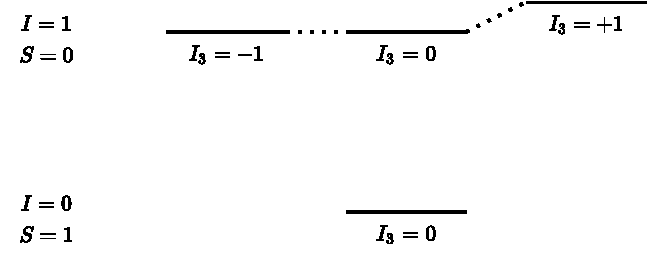
\includegraphics{prob5a.drawio.pdf}
			\end{center}
		
			\item Similarly, \begin{center}
				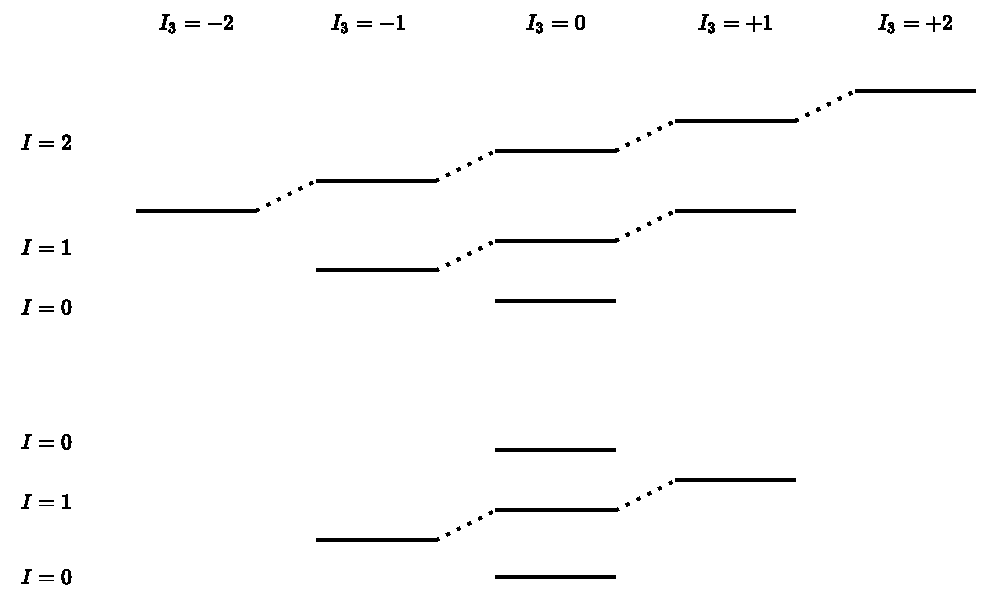
\includegraphics[width=\linewidth]{prob5b.drawio.pdf}
			\end{center}
		
			\item  For \ce{^14 N}, we have 7 neutrons/protons, so we're in an unpaired spin state, so total spin is $1/2$.  For \ce{^14 C} and \ce{^14 O}, we have paired neutrons/protons with a magic number, so the total spin is $S=0$.
			
			The lowest $I$ singlet ($I=0$) would have spin $S=1$, and the triplet ($I=1$) would have $S=0$.
			%It's similar to the diagram on part (a) as we're just swapping between $\pm1$ proton and neutron. It's analogous to the diagram in part (a)
		\end{enumerate}
	
		\pagebreak
		
		\item One possibility is $\Sigma^+$,
		\begin{center}
			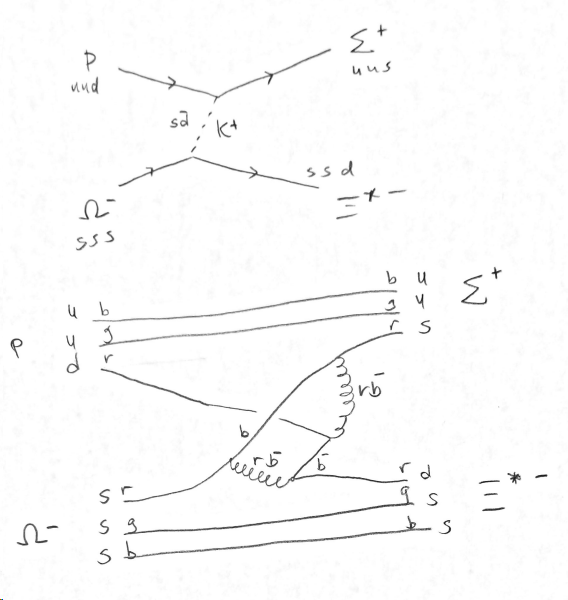
\includegraphics[width=0.7\linewidth]{prob6}
		\end{center}
				
		\item I think there is a typo on the $\mu^-$-decay, since charge wasn't conserved, so I'm assuming it should've gone to an $e^-$.
		
		\begin{minipage}{0.5\textwidth}
			\begin{align*}
				\pi^+ & \to \pi^0 + e^+ + \nu_e \\
				\mu^+ & \to e^+ + \nu_e + \bar{\nu}_\mu \\
				\mu^- & \to e^- + \bar{\nu}_e + \nu_\mu \\
				K^+ & \to \pi^0 + e^- + \bar{nu}_e \\
				\bar{K}^0 & \to \pi^0 + e^- + \bar{\nu}_e \\
				\Sigma^- & \to n + \mu^- + \bar{\nu}_\mu \\
				\Sigma^+ & \to \Lambda^0 + e^+ + \nu_e \\
				D^0 & \to K^- + \pi^0 + e^+ + \nu_e
			\end{align*}
		\end{minipage}
		\begin{minipage}{0.5\textwidth}
			\begin{align*}
				\bar{\nu}_e + p & \to n + e^+ \\
				\nu_e + \ce{^37 Cl} & \to \ce{^37 Ar} + e^- \\
				\nu_\mu + p & \to \mu^- + p + \pi^+ \\
				\nu_e + n & \to e^- + p \\
				\ce{^3 H} & \to \ce{^3 He} + e^- + \bar{\nu}_e \\
				\pi^+ & \to \mu^+ + \nu_\mu \\
				\pi^- & \to e^- + \bar{\nu}_e \\
				\tau^- & \to \pi^- + \pi^0 + \nu_\tau
			\end{align*}
		\end{minipage}
		
		\pagebreak
		
		\item \begin{enumerate}
			\item  ~~ \\ \begin{minipage}{0.5\textwidth}
				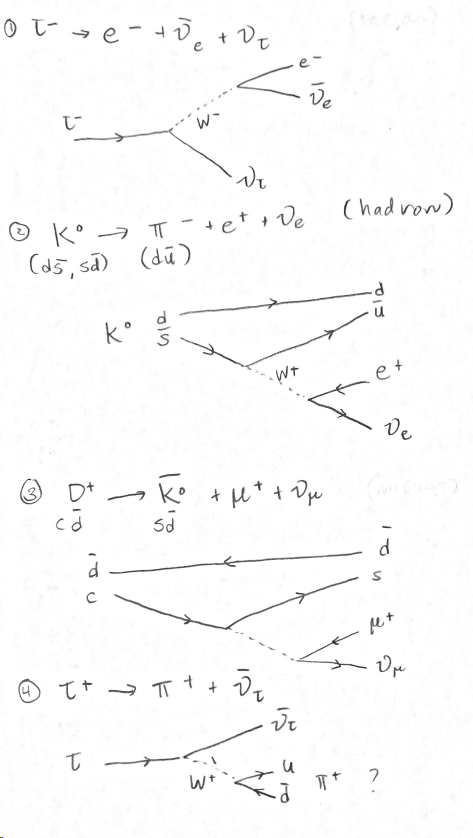
\includegraphics[width=\linewidth]{prob8a1}
			\end{minipage} \begin{minipage}{0.5\textwidth}
			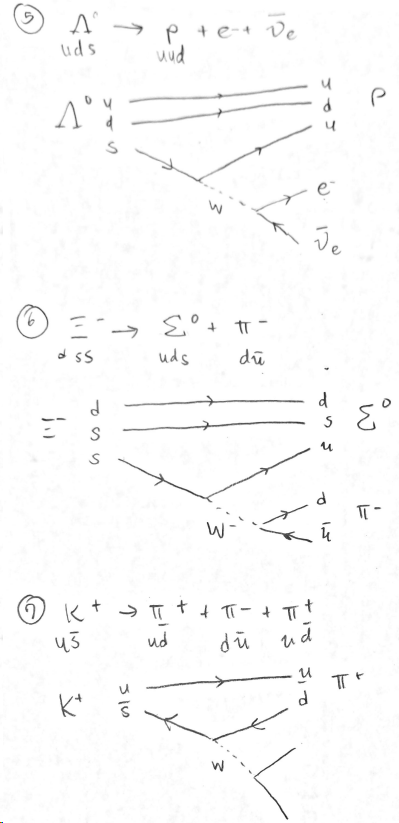
\includegraphics[width=\linewidth]{prob8a2}
			
		\end{minipage}
			
			\pagebreak
			
			\item ~ \\
			\begin{center}
				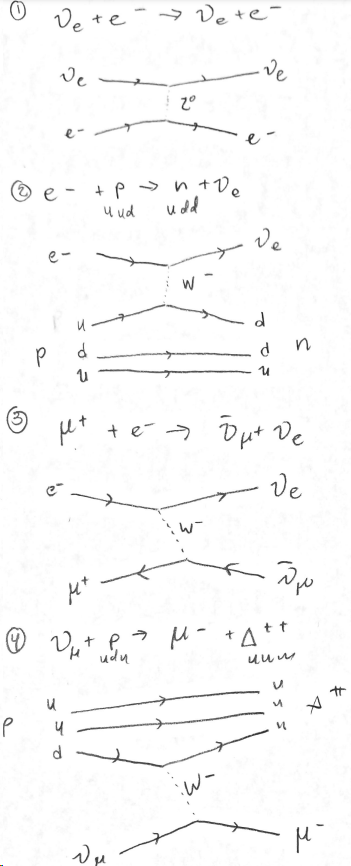
\includegraphics[width=0.6\linewidth]{prob8b}
			\end{center}
		\end{enumerate}
		
		\pagebreak
		
		\item \begin{enumerate}
			\item Under quark exchange, $\zeta_\mathrm{flavor}$ and $\chi_\mathrm{spin}$ are symmetric, so $\phi_\mathrm{color}$ \textit{must} be antisymmetric to fulfill the Pauli exclusion principle.
			
			\item It expands to that since it must includes all combinations of the symmetric quark ordering.
			
			\item For the ${\Sigma^*}^0$ particle, we have to include all permutations, so omitting all the spins (all spin $\uparrow$) and the normalization coefficient, \begin{align*}
				\ket{uds} + \ket{sud} + \ket{dsu}
				- \ket{sdu} - \ket{dus} - \ket{usd}
			\end{align*}
			
			\item The flavor-spin term can't be antisymmetric since the color term is already antisymmetric. This would mean the overall wavefunction is symmetric.
			
			\item Flavor and spin can't treated as separate functions and has to be treated as a single function of \textit{both} flavor and spin.
			
			\item No, as the flavor part for $uuu$, $sss$, $ddd$ is symmetric and the spin part would be symmetric for a spin-1/2 baryon, as $S=0$. This would mean the total wavefunction is symmetric, which cannot be the case. 
			
		\end{enumerate}
	
		
		\item \begin{enumerate} % wyatt
			\item For the time-dependence, we can use $e^{-i E t / \hbar}$ on each state, \begin{align*}
				\psi_\mu (x, t) & = \psi_1 e^{-iE_1 t / \hbar}  \cos \theta + \psi_2 e^{-iE_2 t / \hbar} \sin \theta.
			\end{align*}
		
			\item (I worked with Wyatt on this part.) For the orthogonal electron neutrino wavefunction, \begin{align*}
				\psi_e (x, t) & = -\psi_1 e^{-iE_1 t / \hbar}  \sin \theta + \psi_2 e^{-iE_2 t / \hbar} \cos \theta.
			\end{align*}
			Solving for each $\psi_i$ in terms of $\psi_\mu$ and $\psi_e$, \begin{align*}
				\psi_1 & = \left[ \psi_\mu \cos \theta - \psi_e \sin \theta \right] e^{-i E_1 t / \hbar} \\
				\psi_2 & = \left[\psi_\mu \sin \theta + \psi_e \sin \theta\right] e^{-i E_1 t / \hbar}.
			\end{align*}
			Then, the muon wavefunction can be written \begin{align*}
				\psi_\mu & = \psi_1 e^{-iE_1 t / \hbar}  \cos \theta + \psi_2 e^{-iE_2 t / \hbar} \sin \theta \\
					& =  \left[ \psi_\mu \cos \theta - \psi_e \sin \theta \right] e^{-i 2E_1 t / \hbar} \cos \theta + \left[\psi_\mu \sin \theta + \psi_e \sin \theta\right] e^{-i 2E_1 t / \hbar}   \sin \theta
				\intertext{Looking at just the electron coefficients in the muon wavefunction, the probability is}
				P(\mu \to e) & = \left[- \sin \theta \cos \theta e^{-i2E_1 t / \hbar} + \sin \theta \cos \theta e^{-i2E_2 t / \hbar}\right]^2 \\
					& = 
						\sin[2](\theta)
						\cos[2](\theta)
						\left(
							e^{-i 2 E_2 t / \hbar}
							- e^{-i 2 E_1 t / \hbar}
						\right)^2.
			\end{align*}
%			I think the probability of the muon neutrino turning into an electron neutrino is given by the projection $\braket{\psi_e}{\psi_\mu}$? So, \begin{align*}
%				\braket{\psi_e}{\psi_\mu} & = \int \psi_e^* \psi_\mu \dd[3]{\bvec{r}}
%				\intertext{Since $\psi_1$ and $\psi_2$ are orthogonal, we can omit the cross terms in the product,}
%					& = \int  (-1)\psi_1^*\psi_1 e^{i E_1 t / \hbar} e^{-i E_1 t / \hbar} \cos \theta \sin \theta  \\
%					& \qquad + \psi_2^* \psi_2 e^{i E_2 t / \hbar} e^{-i E_2 t / \hbar} \sin \theta \cos \theta\dd[3]{\bvec{r}} \\
%					& = 
%			\end{align*}
		\end{enumerate}
	
	\end{enumerate}
\end{document}